%% -*- mode: latex; -*-

Formally evaluating the effectiveness of a meta-toolkit for VA is
complex. Arguably the most convincing method would require two groups
of programmers of equivalent skills to implement the same set of
VA programs with and without Obvious. Then, a judgment
could be made from the time spent and the quality of the results. This
methodology has been used to assess IVTK~\cite{InfoVis} with students
but is impractical for real VA applications that are
more complex and would not fit the scope of student projects.

Another method --- used to validate Prefuse~\cite{Prefuse} -- would be
to re-implement complex VA applications using Obvious
and assess the results, again in term of time and quality. This is
what we have done and we report on our results here.

\subsection{Coding applications with Obvious}

This section shows how Obvious can implement common applications in
infovis such as the creation of a scatter-plot or of
a network visualization.  These examples explain how to combine
Obvious components to build an application, how to create data
structure and spot patterns to use.  The first use-case concerns the
coding of a network visualization with the Obvious-IVTK
implementation and the second based on the coding of a scatter-plot by
combining component from different Obvious implementations.

For both examples and more generally for every creation of an Obvious
application, developers have to follow the following steps:

\paragraph{Step 1:} creation of an Obvious data structure, either
directly with a standard constructor or through a factory.  Three ways
exist to fill the data structure:
\begin{enumerate}[noitemsep]
\item wrapping an existing data structure from a targeted toolkit as
  shown in the first example,
\item using an Obvious reader to load an Obvious structure from a well
  known file format (CSV, GraphML...) as shown in the second example,
\item using Obvious methods to directly manipulate the data structure
  (addRow, addNode, addEdge...); an example would be too long for this
  article.
\end{enumerate}

\paragraph{Step 2:} Creation of an Obvious visualization from the
created data structure and additional parameters.  This can be done
directly with a class constructor or through a factory.  The
parameters allow customization of the Obvious monolithic components.
As shown in the second example, it is possible to use the data
structure from one Obvious implementation with a visualization from
another.

\paragraph{Step 3:} Creation of an Obvious view with the created
visualization directly with a constructor or through a factory.

\begin{lstlisting}[caption={Visualizing a graph with Obvious},label=codeSample1]
// Creates the graph structure. First, set the factory to use (ivtk).
// Then loads the native data structure, and get a factory instance.
// Finally, calls the convenient method of the factory.
System.setProperty("obvious.DataFactory",
    "obvious.ivtk.data.IvtkDataFactory");
infovis.Graph g = Algorithms.getGridGraph(10, 10);
DataFactory factory = DataFactory.getInstance()
Network network = factory.createGraph(g);

// Creates the associated visualization using the
// factory for visualization. No predicates and extra
// parameters are given to the constructor.
Visualization vis = new IvtkVisualizationFactory()
    .createVisualization(network, null, "network", null);

// Creates the view. No predicates and extra parameters are given to
// the constructor.
View view = new IvtkObviousView(vis, null, "graphview", null);
// Standard Java window creation
JFrame frame = new JFrame();
JScrollPane panel = new JScrollPane(view.getViewJComponent());
frame.add(panel);
frame.pack();
frame.setVisible(true);
\end{lstlisting}

\begin{lstlisting}[caption={Combining different Obvious implementations to display a scatter-plot},label=codeSample2]
// Defines the data factory to use,
// Obvious-Prefuse will be used for the data structures.
System.setProperty("obvious.DataFactory",
    "obvious.prefuse.PrefuseDataFactory");
// Creates an Obvious CSV reader and loading an
// Obvious table
CSVImport csv = new CSVImport(new File("example.csv"), ',');
Table table = csv.loadTable();

// Creates the parameter map for the monolithic object.
Map<String, Object> param = new HashMap<String, Object>();
param.put("x", "id"); // xfield
param.put("y", "age"); // yfield

// Creates the visualization then the view. No predicates are given to
// the constructor.
Visualization vis = new IvtkScatterPlotVis(table, null, "plot", param);

View view = new IvtkObviousView(vis,  null, "plot", null);
// Standard Java window creation
...
\end{lstlisting}

\subsection{Integration of Weka}

Weka~\cite{Weka} is a suite of machine-learning algorithms and data
structures widely used to design machine-learning applications.  
The obviousx package of Obvious supports two mechanisms to build the
main data structure of Weka (called ``Instances'') from an Obvious
Table:

\begin{itemize}[noitemsep]
\item an Obvious table can be copied into a Weka ``Instances'', which
  is a data structure specially optimized for the fast execution of
   machine learning algorithms.  With this approach, running-time is
   optimized.
\item an Obvious table can be wrapped as a Weka ``Instances'': the
  Instances translates its methods calls into Obvious equivalents.
  With this approach, memory-footprint is optimized.
\end{itemize}

Both methods are equivalent in terms of lines of code and can be
applied to the same machine learning algorithms from Weka.  For
example, wrapping the table from the code sample \ref{codeSample2}
into a Weka ``Instances''  requires the following line:

\begin{lstlisting}[caption={Wrapping an Obvious Table into Weka Instances},label=wekaExample]
Instances inst = new ObviousWekaInstances(table, "Instances");
\end{lstlisting}

%% To wrap the Obvious structure, the constructor simply needs as
%% argument the Obvious table and a name for the weka Instances.  

This ``Instances'' can be used by all the machine-learning algorithms
defined in Weka.  Creating this wrapper took about three days to one
developer who knew Obvious well but was discovering Weka.

This example demonstrates an important gain of Obvious: a toolkit with
a binding in Obvious can immediately benefit from a substantial set of
additional features, such as Weka for advanced machine-learning
capabilities and several format converters.  Conversely, developers of
new analysis algorithms could port them to use Obvious data structures
so that they become usable by a substantial number of toolkits and
application programmers to build VA systems.


\subsection{EdiDuplicate}

INRIA maintains a repository called
HAL-INRIA\cite{HAL} to store, index and give
access to its publications.  Entering publications is a manual process
done by researchers who make mistakes.  These mistakes can result in
duplicated authors, institutions, or articles. Thus, INRIA needs to
clean the HAL database with tools that can detect potential duplicates
and ask skilled users to resolve them.  Currently, INRIA leaves that
task to librarians with very primitive tools.

EdiDuplicate is a system designed to detect and merge duplicated
entities in the HAL-INRIA publication database that has been built
with Obvious; it is an adaptation of the D-Dupe software~\cite{DDupe}
with extensions to cover needs specific the HAL-INRIA
database\cite{HAL} to perform other operation in a workflow.

Each time a new entity is created in the database, multiple similarity
metrics are automatically computed between this entity to all the ones
already in the database.  This information is loaded on an Obvious
table and displayed, as shown on the left pane of
Figure~\ref{fig:ediduplicate} using a standard Java table.  Each row
refers to one pair of names and the columns contain the multiple
similarity measures with a green-red color coding; the table that can
then be sorted according to any column order.

When a pair is selected by clicking on a row, a network view is created
that visualize the neighborhood network of the pair of entities, as
shown on the right of Figure~\ref{fig:ediduplicate}.  The
neighborhood is computed from publication data: for a target entity,
it contains all the entities already connected to it through
co-authorship relations.  This information helps the user decide if
the pair of entities has to be merged.

\begin{comment}

This problem has already been addressed by at least two communities:
the database community, which calls it the ``Record Linkage'' or
``Entity Resolution'' problem, and the VA community with
the D-Dupe tool~\cite{DDupe}.  D-Dupe uses similarity metrics between
entity names and infovis techniques to show a rich
set of information to the librarian to make a decision whether two
entities are the same or different.  However, since D-Dupe does not
connect to the workflow of HAL, we used Obvious to build a similar
tool that we called EdiDuplicate.
\end{comment}

\begin{figure}[!h]
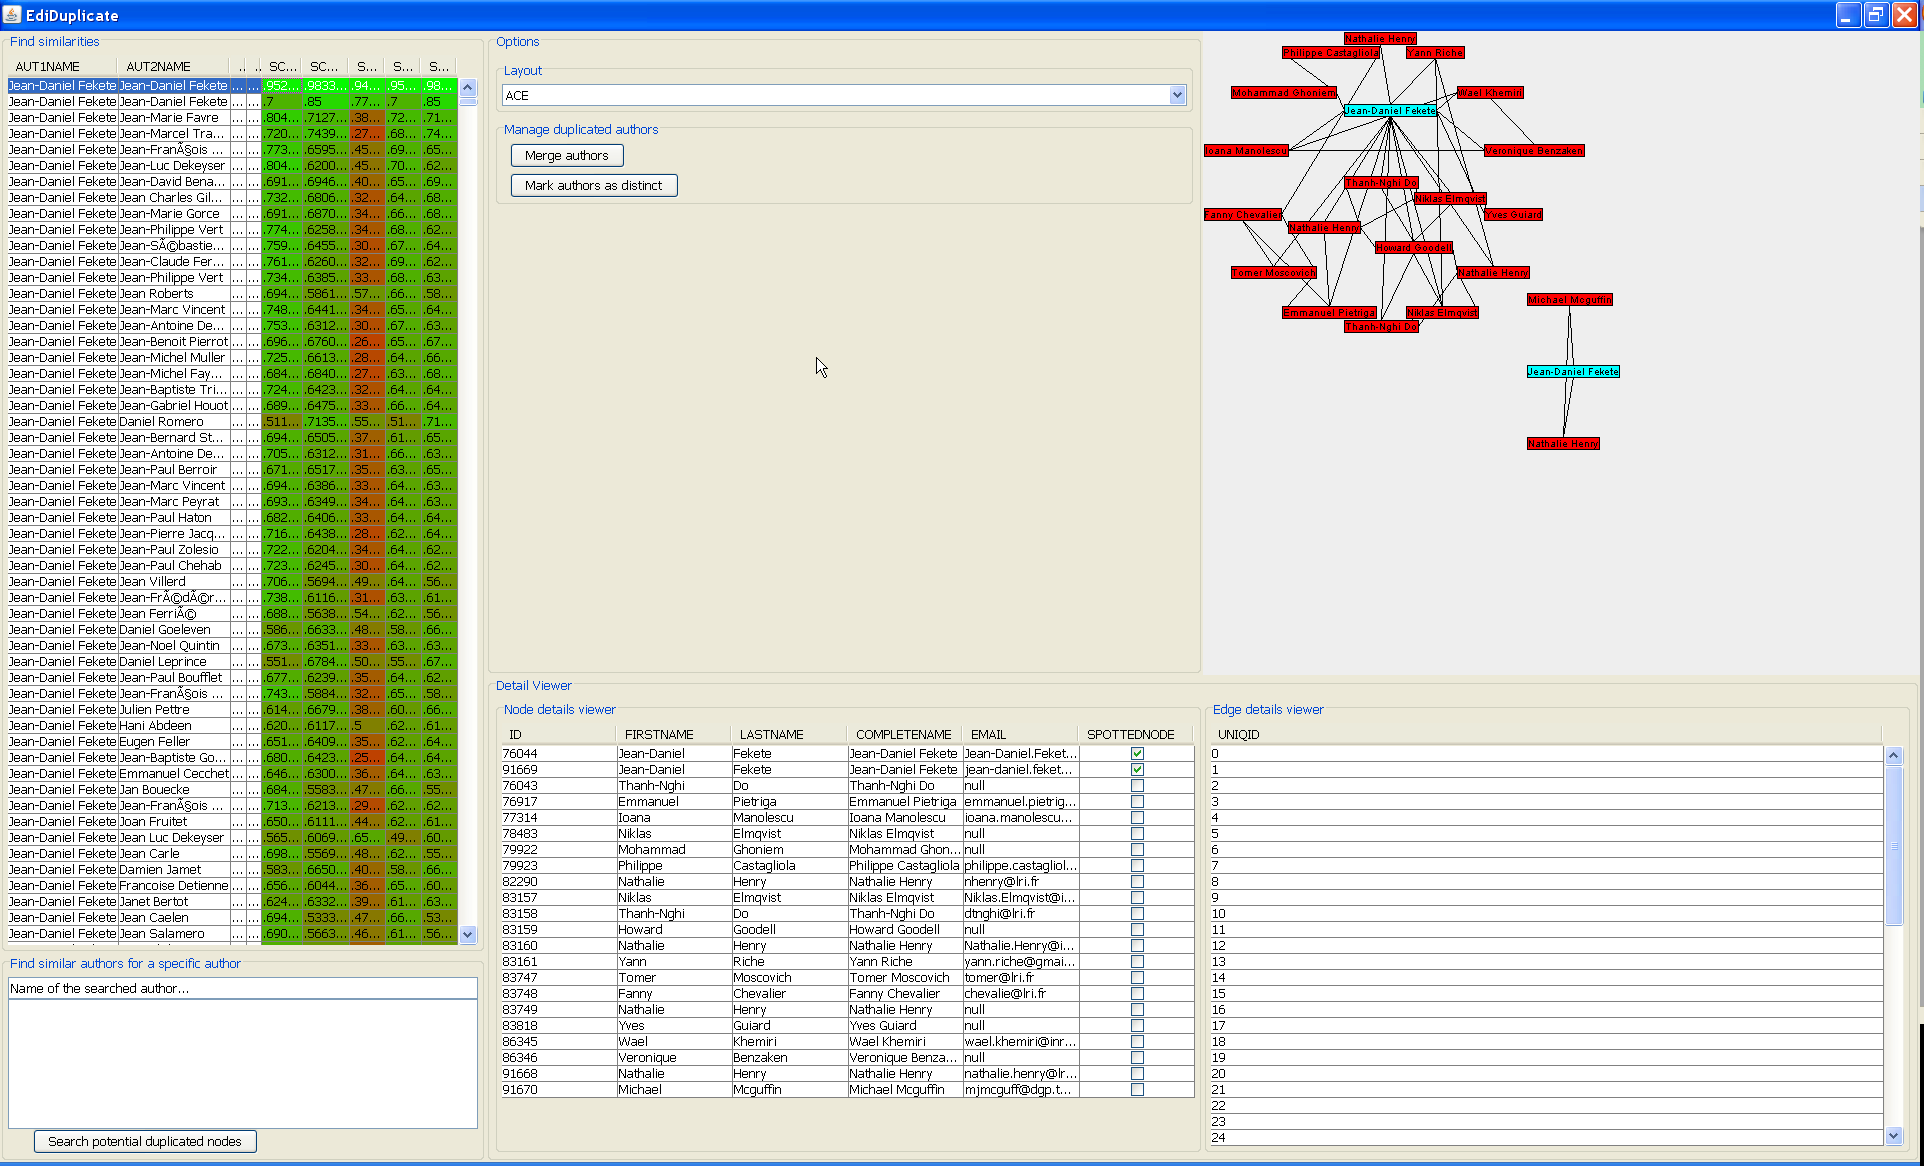
\includegraphics[width=\columnwidth]{figures/ediduplicate}
\caption{The EdiDuplicate application}
\label{fig:ediduplicate}
\end{figure}

The application mainly combines Obvious components and Swing
components (derived from Obvious structures). For the data model, an
Obvious Network is used with the IVTK implementation of Obvious; the
visualization and the view parts are also provided by this
implementation.  Building this application took less than a week.

\subsection{DBMS Caching Tables}
\label{dbmscachingtable}

We have extended the JDBC implementation of Obvious to allow caching
and notification management directly from a table stored in a DBMS.
Currently, this mechanism works with the Oracle and MySQL DBMSs.  The
Obvious data table component reads data on demand from a table in the
DBMS, stores it in memory and serves it from memory while keeping a
bidirectional link with the DBMS.  When the DBMS table is modified
from any application, a database trigger is invoked that notifies the
Obvious table implementation that some rows are invalid.  They are
then flushed from memory and will be read again when the application
needs it.  The communication between the DBMS and the Obvious
component is done through a fast network connection (UDP packets).
Oracle provides a standard API to send UDP packets whereas we had to
add an extension written in C to MySQL to support them (200 lines of
C).

\begin{comment}
The need to create DBMS caching data table appears during the development
of Ediflow, a Scientific Workflow system for VA~\cite{Ediflow}.
Ediflow is organized around a DBMS (Oracle) and runs modules processing
large amount of data stored in the DBMS. Ediflow is a distribued system
allowing workflows to be distributed on several platforms.

When running a visualization component with Ediflow, all its resulting
visual attributes are stored in a table of the DBMS called
``VISUALATTRIBUTES''. This table is then used to create and maintain
views on other platforms using Ediflow.

To set up and maintain thoses view, in-memory caching tables are needed
to only select in ``VISUALATTRIBUTES''  data useful for those views
and to locally store it.
\end{comment}

The cached tables are implemented using Obvious (different bindings
have been used: Prefuse, IVTK, JDBC and JUNG). Several applications have
been built around Obvious DBMS caching tables; one of them is
presented in the next section.

\subsection{Network Visualization on a Large Wall}

INRIA shares with other institutions a Wall-Size display called
WILD~\cite{Wild} made of 32 high-resolution 32" screens.  Using
Obvious, we have developed an application for visualizing
co-authorship networks on WILD.  WILD is made of 16 machines serving 2
screens each and connected to a fast network.

Our application uses a client-server approach: the server program
loads the network using Obvious, computes its layout and stores the
result as a set of graphic primitives in a database table using an
Obvious-JDBC data table.  For each screen, one client program is
launched that uses the DBMS caching data-structure to load the
relevant portion of the nodes and links: the area that is visible on
the portion of the screen managed by the client.

An Oracle DBMS is used to store publications data in two tables: one
for the authors (containing id and name) and one for the publications
(containing pairs of publication id and author id).

Our application uses Obvious-Prefuse in the server and in the clients,
with Obvious-caching data-structures.  A polylithic architecture is
particularly well suited to this kind client-server approach sharing
the visualization through the network.

Since cached tables are synchronized with the DBMS, the whole pipeline
is dynamic: when a data table containing the network is modified
(e.g. a new author is added), it is reloaded by the server, the layout
is recomputed by Prefuse and the visual table is stored in the DBMS.
When the DBMS visual tables is changed, the clients are notified and
they reload and redisplay their content.

Designing the application boiled down to having a first version using
Obvious-Prefuse in memory, then changing the data tables to use the
JDBC caching, then changing the visualization to store its results in
the database through an Obvious-JDBC table and then implementing the
clients.  A step-by-step development where the application logic can
be tested first on a standard desktop computer and then deployed to a
more specific setup.

\subsection{Implementing a Cross-Toolkit Layout Component}

We have also tested a more advanced usage scenario: devising
a novel layout algorithm and using the Obvious toolkit to make it
available in a variety of toolkits. This layout component is a
generalized treemap algorithm.
%% ~\cite{Treemaps2011}.  [jdf: not yet]
Its interface makes it easy to port as this
algorithm takes as input a data model and renders using a Visitor
design pattern to a renderer object, making it very convenient to
implement across polylithic toolkits such as Prefuse or Discovery.
Considering that the current visualization model is mostly targeted at
enabling monolithic patterns, Obvious in its current state turns out
to be of limited use for our purpose.

Still, we have found that the existing data model and utilities have
made developing our layout algorithm on top of Obvious worthwhile: we
could implement very easily a simple monolithic visualization and
view instances, and relying on the default data model already saves us
time in the development of our prototype, while we have the assurance
that only minimal work may be needed to port our method to the
toolkits targeted by Obvious.


\subsection{Conclusion}

The examples described in this section assess an important strength of
Obvious: it allows a clear separation of concerns in the development
of VA applications with a small memory and performance footprint.  The
data model of the application can be chosen independently from the
visualization components as long as all these components fit the
Obvious model.  From our experience, a large number of the VA
application fit the Obvious model and they will benefit from the
meta-toolkit in term of richness and extensibility.

